\documentclass{beamer}
\usepackage{graphicx} % Allows including images
\usepackage{natbib} 
\usepackage{booktabs} % Allows the use of \toprule, \midrule and \bottomrule in tables


\mode<presentation> 
{
    \usetheme{Madrid}
    
    \usecolortheme{rose}
       
    % Replace footer line in all slides with a slide count 
    \setbeamertemplate{footline}[page number]
    
    % Remove navigation symbols from the bottom
    \setbeamertemplate{navigation symbols}{} 
}

% ---------------
%	TITLE PAGE
% ---------------

% Short title appears on bottom of all slides
\title[Writer Identification]{EDGE-BASED DIRECTIONAL FEATURE EXTRACTION FOR WRITER IDENTIFICATION}
\author{Himanshu Kumar Keshri  \\ {\small 218CS1084}} % Your name

\institute[NIT Rourkela] 
{
	\small Guided by : Dr. R.K. Mohapatra
	\\
	\huge National Institute of Technology, Rourkela \\
	\medskip
}
\date{} % Date, can be changed to a custom date


\begin{document}
	
	%%%%%%%% Title Page %%%%%%%%%%%%%%%
	\begin{frame}
		\titlepage
		\thispagestyle{empty}
	\end{frame}

	\begin{frame}
		\frametitle{INTRODUCTION}
		\begin{itemize}
			\item Authors : Marius Bulacu, Lambert Schomaker, Louis Vuurpijl 
				\begin{figure}
				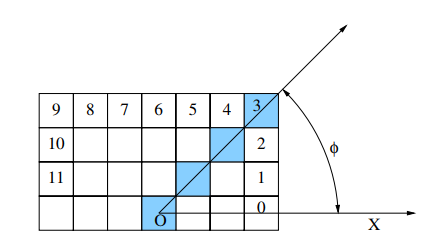
\includegraphics[width=0.6\linewidth]{edgedirection.png}
				\caption{\ref{fig:edgedirection} Extraction of edge-direction distribution}
				\label{fig:edgedirection}
			\end{figure}
			\item Each edge pixel in the middle of the square.
			\item To avoid redudancy, only uppper two quadrants are checked
			\item If the length of edge is $l$ then number of feature extracted is 
			\[ {n}= 5+4({l}-2)\]
		\end{itemize}
	\end{frame}

	\begin{frame}
		\frametitle{IMPLEMENTATION}
			\begin{figure}
				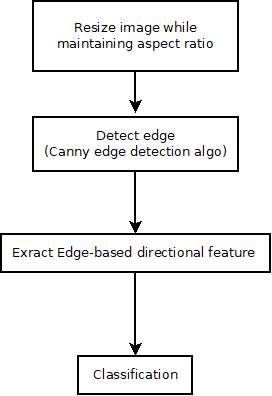
\includegraphics[height=0.8\textheight]{flowchart.png}
				\caption{\ref{fig:flowchart} Flowchart}
				\label{fig:flowchart}
			\end{figure}
	\end{frame}

	\begin{frame}
		\frametitle{IMPLEMENTATION}
		\begin{itemize}
			\item Dataset - IAMDB
			\item 5 Writer where each writer have written 10 forms
			\item features are extracted both sentence level and word level
		\end{itemize}
	\end{frame}

	\begin{frame}
		\frametitle{RESULTS}
		\begin{table}
			\centering
			\label{tab:evaluation}
			\setlength{\tabcolsep}{2pt}
			\begin{tabular}{|p{1cm}|p{2cm}|p{2cm}|p{2cm}|p{2cm}|p{2cm}|}
				\hline
				\textbf{No.} & \textbf{Edge length} & \textbf{Feature extraction level} & \textbf{Model}  & \textbf{Accuracy} & \textbf{Remark} \\ \hline
				1 & 4 & Sentence & MLP(HL - 100, alpha-0.0005, epoch-50) & 28.5\% & less no of data generated \\ \hline
				2 & 4 & Word & MLP(HL - 100, alpha-0.0005, epoch-50) & 75.72\% & word level features are better than sentence level \\ \hline
				2 & 5 & Word & MLP(HL - 100, alpha-0.0005, epoch-50) & 72.67\% & increasing edge length is not helpful\\ \hline
			\end{tabular}
			\caption{Evaluation of different models}			
		\end{table}
	\end{frame}



\end{document}





